\chapter{Narukvica}
\label{pog:bracelet}
Svrha narukvice je prikupljanje biomedicinskih parmetara korisnika i njihovo slanje na obradu na glavnoj ploči. Biomedicinski parametri koji će se promatrati su brzina otkucaja srca putem fotopletizmografskog senzora (PPG) i vodljivost kože, odnosno elektrodermalna aktivnost. Promjena elektrodermalna aktivnost je dobar pokazatelj stresa u korisnika \cite{edr}, a osobe sa poremećajem tečnosti govora pokazuju značajno smanjenje brzine otkucaja srca u stresnim situacijama u odnosu na osobe bez takvih poremećaja \cite{ALM2004123}.

Što se tiče zahtjeva na napajanje narukvice, situacija je ista kao i kod glavne ploče, uz drugačiju potrošnju. Tako da izrada pločice za narukvicu predstavlja mogućnost ispravljanja grešaka nastalih tijekom dizajna napajanja glavne ploče. Narukvica također mora imati mogućnost bežične komunikacije. S obzirom na ograničenje veličine ploče maknuti su kratkospojnici i testne točke.

\section{Bežična komunikacija}
Shema bežične komunikacije na narukvici (slika \ref{slk:BR_WIRELESS}) je veoma slična onoj na glavnoj ploči (slika \ref{slk:WIFI}), uz nedostatak kratkospojnika. Još jedna promjena dolazi u obliku % napiši nešto u vezi autoprograma
\begin{sidewaysfigure}[htbp]
    \centering
    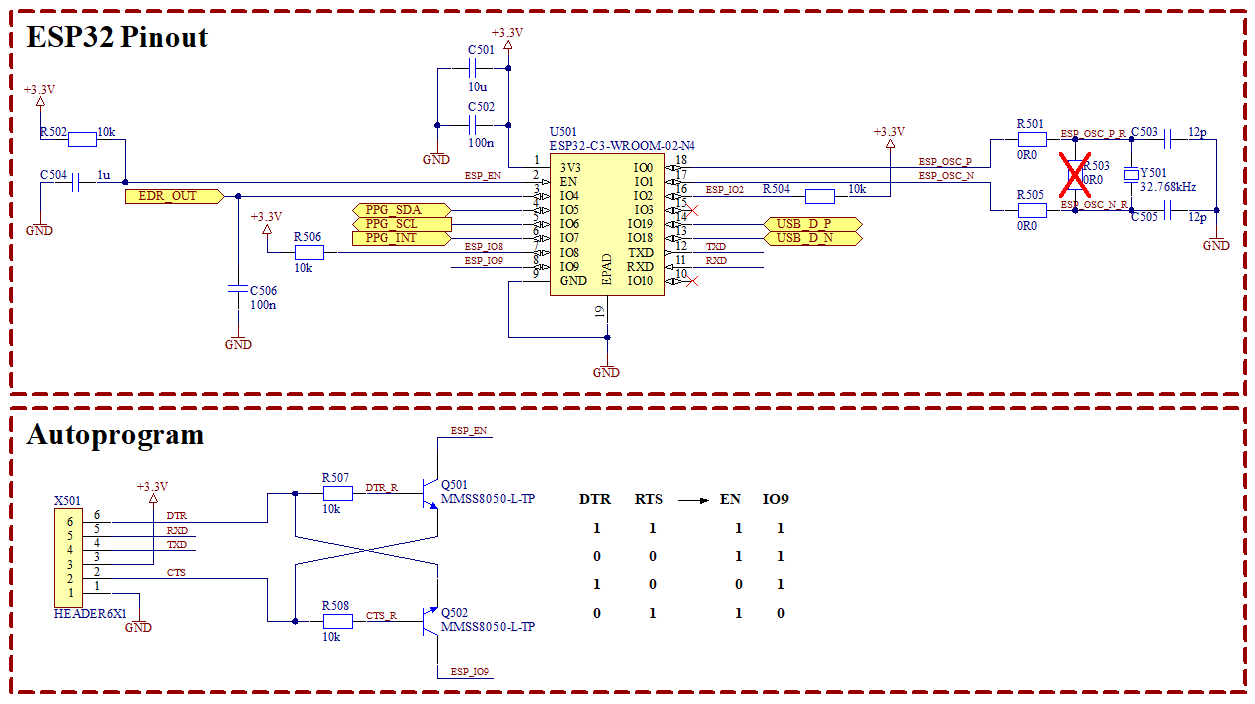
\includegraphics[width=1\textwidth]{Figures/BR_WIRELESS.png}
    \caption{Shema bežične komunikacije narukvice}
    \label{slk:BR_WIRELESS}
\end{sidewaysfigure}

\section{Fotopletizmografski senzor}
